%%%%%%%%%%%%%%%%%%%%%%%%%%%%%%%%%%%%%%%%%%%%%%%%%%%%%%%%%%%%%%%%%%%%%%%%%
%Objetivo: Realizar uma pesquisa com profissionais envolvidos em manutenção de
%		   software a fim de verificar a situação atual das funcionalidades
%		   oferecias pelas FGRM.
%Autor: Vagner Clementino<vagnercs@dcc.ufmg.br> e
%		Rodolfo Resende<rodolfo@dcc.ufmg.br>
%Data Criação: sex fev  3 19:57:56 BRST 2017
%Data Modificação: qui abr  6 20:33:42 -03 2017
%Data Revisão: qui abr  6 21:01:54 -03 2017
%%%%%%%%%%%%%%%%%%%%%%%%%%%%%%%%%%%%%%%%%%%%%%%%%%%%%%%%%%%%%%%%%%%%%%%%%%
\chapter{Levantamento por Questionário com Profissionais}
\label{ch:pesquisa-profissionais}

\section{Introdução}
\label{sec:pesquisa-profissionais-intro}

Um levantamento por questionários, conhecido na literatura como
\textit{Survey}, é uma abordagem de coleta e análise de dados em que os
participantes respondem a perguntas ou declarações que foram desenvolvidas
Este tipo de estudo permite que os pesquisadores generalizem as crenças e
opiniões de uma população mediante os dados coletados de um subconjunto do
público-alvo (amostra). No trabalho conduzido por
Kasunic~\cite{kasunic2005designing} são apresentadas uma sequência de etapas a
serem seguidas no processo de condução deste tipo de trabalho:

\begin{enumerate}
\item{Identificar os objetivos da pesquisa}
\item{Identificar e caracterizar o público-alvo}
\item{Elaborar o plano de amostragem}
\item{Elaborar e escrever um questionário}
\item{Aplicar questionário de teste ou piloto}
\item{Distribuir o questionário}
\item{Analisar os resultados e escrever o relatório}
\end{enumerate}

Com o objetivo de coletar os aspectos mais importantes das funcionalidades
oferecidas pelas Ferramentas de Gerenciamento de Requisições de Mudança (FGRMs),
do ponto de vista dos profissionais ligados à manutenção de software, realizamos
um levantamento mediante questionário. O planejamento e o desenho do estudo
seguiu as diretrizes propostas nos trabalhos de
Wohlin~\cite{wohlin2012experimentation} e Kasunic~\cite{kasunic2005designing}.
Em especial, no tocante a definição da população e da amostra de interesse
utilizamos o arcabouço (framework) proposto por De Mello e
outros~\cite{de2015investigating, de2014towards}.

A população da pesquisa é a comunidade envolvida com o processo de manutenção de
software e que faça uso de FGRMs. Neste sentido, utilizamos como amostra os
profissionais que estão envolvidos no projeto de código aberto
Python\footnote{\url{http://bugs.python.org/}}. Por outro lado, visando alcançar
profissionais que trabalham em empresas privadas, utilizamos os usuários da
rede social de desenvolvedores Stack
Overflow\footnote{\url{http://stackoverflow.com}}. Neste último caso, estamos
interessados nos usuários da rede que tenham participado de discussões sobre
assuntos relacionados à manutenção de software. A pesquisa foi replicada em uma
empresa pública de software do qual o autor possui vínculo. Maiores detalhes
sobre o processo de escolha das amostras serão discutidos posteriormente.

A importância deste tipo de trabalho está na possibilidade de avaliar se as
pesquisas relativas a evolução das funcionalidades das FGRMs estão em
consonância com as necessidades dos profissionais. Neste sentido é possível
discutir a distância entre o estado da arte e o estado da prática.

\section{Objetivo do Levantamento com Profissionais}
\label{sec:objetivo_da_pesquisa_com_profissionais}

Em linhas gerais, o objetivo desta etapa da dissertação é analisar, através da
percepção e opinião dos profissionais envolvidos em manutenção de software, a
situação das funcionalidades atualmente oferecidas pelas FGRMs, bem como a
adotação das metodologias propostos pelos agilistas no processo de manutenção de
software. Colocando a finalidade do levantamento conforme propõe a metodologia
GQM (Goal, Question e Metric)\cite{gqm}, \textit{o propósito deste estudo é
	avaliar as funcionalidades oferecidas pelas FGRMs e as melhorias propostas
	nas literatura, do ponto de vista dos
	profissionais envolvidos em manutenção de software no contexto de projetos
	de software de código aberto e uma empresas publicas e privadas de
	informática.}

Com intuito de atingir os objetivos propostos foram definidas as seguintes
questões de pesquisa:

\begin{description}
	\item[Questão 01] Qual a opinião dos profissionais envolvidos em Manutenção
		de Software com relação as funcionalidades oferecidas atualmente pelas
		FGRM\@?
	\item[Questão 02] Na visão dos profissionais envolvidos em Manutenção de
		Software quais das extensões propostas na literatura teriam maior
		relevância em suas atividades atuais?
	\item[Questão 03] Como as práticas propostas pelos agilistas estão sendo
	utilizadas especialmente no processo de manutenção de software?
	\item[Questão 04] Como as FGRMs podem ajudar aos times devotados à manutenção
	de software na prática adotada pelos agilistas?
\end{description}

O desenho da pesquisa é detalhado na próxima seção onde discutimos a estrutura
do questionário bem como a amostra da população que foi utilizada.

\section{Desenho e Metodologia da Pesquisa com Profissionais}
\label{sec:desenho_da_pesquisa_com_profissionais}

\subsection{Conceitos Básicos}

Estudos primários em Engenharia de Software (SE), como os levantamentos por
questionário, são muitas vezes conduzidos em amostras estabelecidas por
conveniência~\cite{sjoberg2005survey, dybaa2006systematic}. Um desafio no
estabelecimento de amostras representativas, especialmente em Engenharia de
Software, é a identificação de fontes relevantes e disponíveis que permitam
criar as amostragem~\cite{de2014towards}. Uma alternativa é a utilização de
fontes disponíveis na Internet, como as rede sociais, para aumentar o tamanho da
amostra~\cite{de2013would}. Outra fonte que pode aumentar a significância das
amostras são os projetos de código e seus respectivos artefatos.

O nosso levantamento com profissionais consistiu de um estudo exploratório sem
uma hipótese prévia. Idealmente, este levantamento deveria ser aplicado em todos
os profissionais envolvidos em desenvolvimento e manutenção de software e que
tenham feito o uso razoável de alguma FGRM. Naturalmente não é possível alcançar
aquela população. Desta forma, foi utilizada uma estratégia de amostragem de
\textit{conveniência} onde o questionário foi aplicado em dois grupos distintos.
Neste tipo de amostragem a seleção de indivíduos é realizada por conta de sua
facilidade de acesso ou proximidade~\cite{marshall1996sampling}. Maiores
detalhes sobre o processo de amostragem serão discutidos na
Seção~\ref{subsubsec:fontes_amostragem}.

O trabalho de Mello e outros~\cite{de2014towards} apresenta um
arcabouço (framework) conceitual para a determinação de fontes adequadas para
amostragens de profissionais em levantamentos na área de Engenharia de Software.
Decidimos utilizar alguns aspectos deste arcabouço para discutir a adequação da
nossa amostra. O modelo proposto inclui além dos conceitos estatísticos
tradicionalmente utilizados em levantamentos com questionário, tais como
público-alvo, população, amostragem e unidade de
observação~\cite{thompson2012sampling}, discute conceitos relacionados com
\textit{Fonte de Amostragem, Unidade de Pesquisa, Plano de Pesquisa e Estratégia
	de Amostragem}.

%A \textit{Unidade de Observação} é a entidade que é estudada em determinado
%experimento~\cite{wohlin2012experimentation}. Uma Unidade pode ser produtos,
%processos, recursos, modelos, métricas, teorias ou pessoas. Uma \textit{Unidade
	%de Pesquisa} caracteriza como uma ou mais \textit{Unidade de Observação}
%podem ser recuperadas de uma \textit{Fonte de Amostragem} específica. O
%\textit{Plano de Pesquisa} descreve como \textit{Unidades de Pesquisa} serão
%sistematicamente recuperadas de uma Fonte de Amostragem e avaliadas para compor
%a amostragem da pesquisa. Finalmente, a Estratégia de Amostragem descreve as
%etapas que devem ser seguidas para definição da amostragem e recrutamento de
%indivíduos que participarão do estudo.

No trabalho de De Mello e outros~\cite{de2014towards} afirma-se que uma Fonte
de Amostragem deve ser organizada utilizando um sistema de banco de dados
possibilitando a extração de subconjuntos da amostra disponível da população.
Sendo assim, os autores discutem que no caso de uma Fonte de Amostragem ser
considerada válida para um contexto de pesquisa específico, pode-se concluir que
as amostras podem ser extraídas desta fonte também podem ser consideradas
válidas.

%\begin{description}
	%\item[ER1] Uma Fonte de Amostragem não deve representar intencionalmente um
		%subconjunto segregado do público-alvo, ou seja, dado um público-alvo
		%\textit{``X''}, não seria adequado pesquisar por unidades na Fonte
		%intencionalmente desenhada para compor um subconjunto específico de
		%\textit{``X''}.
	%\item[ER2] Uma Fonte de Amostragem não deve apresentar qualquer viés em
		%incluir na sua base de dados determinados subconjuntos do público-alvo.
		%Critérios desiguais para inclusão de Unidades de Pesquisa significam
		%oportunidades desiguais para oportunidades de amostragem.
	%\item[ER3] Todas as Unidades de Pesquisa das amostras e suas Unidades de
		%Observação devem identificados por de forma única.
	%\item[ER4] Todas as amostragem de determinada Unidade de Pesquisa devem ser
		%acessíveis. Se houver unidades de pesquisa ocultas, não é possível
		%contextualizar a população.
%\end{description}

%O estudo realizado por de Mello~\cite{de2014towards} cita outros requisitos que
%são definidos como desejáveis que estão relacionados com amostragem, clareza e
%integridade da amostra. Contudo, neste trabalho, a Fonte de Amostragem foi
%valiada apenas pelos ERs.

\subsection{Metodologia}
\label{subsec:pesq_metodologias}

No caso deste levantamento por questionário, o público-alvo é o conjunto de
profissionais que trabalham com manutenção de software e que tenham uma razoável
experiência de uso das FGRMs. A caracterização e estratificação da população que
temos interesse não é simples. Neste sentido, é difícil dizer que um extrato com
uma certa experiência com FGRMs é mais relevante do que outro com maior tempo de
uso deste tipo de ferramenta ou ainda questões como processo de software ou
linguagem de programação. Salvo melhor juízo, todos os desenvolvedores de código
aberto e código proprietário, que de alguma forma tenham utilizado alguma FGRM,
podem podem ser relevantes nesta investigação. Elaboramos um Plano de Pesquisa
onde excluímos participantes conforme critérios que serão detalhados a seguir.

\subsubsection{Fontes de Amostragem}
\label{subsubsec:fontes_amostragem}

Uma \textit{Fonte de Amostragem} consiste de um banco de dados, que não
necessariamente é automatizado, em que um subconjunto válido da população pode
ser sistematicamente recuperado, além de permitir a extração aleatória de
amostras da população de interesse~\cite{de2014towards}. Utilizamos neste estudo
as duas Fontes de Amostragem exibidas na Tabela~\ref{tab:fontes-amostragens}.
Na primeira fonte, temos a expectativa de encontrarmos indivíduos ligados ao
desenvolvimento da plataforma Python correspondam ou representem profissionais
do extrato de código aberto. A segunda fonte, FA02, corresponde a indivíduos com
interesse na rede social denominada Stack Overflow e neste caso devemos
encontrar um perfil mais abrangente de desenvolvedores e mantenedores de
software\footnote{Não colocamos esforço em tentar distinguir se o foco de
	atividade do usuário do Stack Overflow é desenvolvimento, manutenção ou
	outra categoria}.

\begin{table}[htpb]
\centering
\resizebox{\textwidth}{!}{%
\begin{tabular}{@{}lllc@{}}
\toprule
\textbf{Identificador} & \multicolumn{1}{c}{\textbf{Fonte de Amostragem}} & \multicolumn{1}{c}{\textbf{URL}} & \textbf{Membros} \\ \midrule
FA01 & Python & https://bugs.python.org/ & $\sim$19 K \\
FA02 & Stack Overflow & https://stackoverflow.com & $\sim$6 M \\ \bottomrule
\end{tabular}%
}
\caption{Fontes de Amostragem utilizadas no levantamento com questionário.}
\label{tab:fontes-amostragens}
\end{table}

A fonte FA01 foi utilizada por apresentar as seguintes características:
\textit{(i)} pelo menos 5 anos de existência; \textit{(ii)} comunidade bem
estabelecida, no sentido de um número relevante e participativo de
contribuidores e usuários; \textit{(iii)} permite acesso aos dados históricos de
suas RMs. Por outro lado, a fonte FA02 foi selecionada por devido à sua
cobertura, que conta com mais de 6 milhões de usuários\footnote{Disponível em
	\url{http://stackexchange.com/sites}. Acessado em novembro de 2016.}.

Conforme anteriormente discutido, este levantamento fez uso de uma amostragem de
conveniência. Embora este tipo de estratégia de amostragem apresentar limitações
devido a natureza subjetiva na escolha da amostra, ela é útil especialmente
quando a randomização não é possível, como no caso de uma população muito grande
ou de difícil caracterização~\cite{boxill1997introduction}. No estudo conduzido
por de Melo e outros~\cite{de2014towards} é apresentam quatro itens denominados
``Requisitos Essenciais'' identificados como \textit{ER1, ER2, ER3 e ER4}. Estes
itens dão validade a uma fonte de amostragem. Nossa avaliação é que nossa fonte
satisfaz bem todos requisitos.

%However, a researcher may not be able to obtain a random or stratified sample,
%or it may be too expensive. A researcher may not care about generalizing to a
%larger population. The validity of non-probability samples can be increased by
%trying to approximate random selection, and by eliminating as many sources of
%bias as possible.

%A convenience sample is a matter of taking what you can get. It is an accidental
%sample. Although selection may be unguided, it probably is not random, using the
%correct definition of everyone in the population having an equal chance of being
%selected. Volunteers would constitute a convenience sample.

\subsubsection{Construção das Fontes de Amostragem}
\label{subsubsec:construcao_fonte_amostragem}

A unidade básica de informação para construirmos as Fontes de Amostragem foram a
lista de RMs disponível em sua respectiva
FGRM\footnote{\url{http:bugs.python.com}} (FA01) e as discussões propostas pelos
usuários (FA02). Em ambos os casos foram coletados os atributos:

\begin{itemize}
	\item Nome do Participante
	\item E-mail do Participante
	\item Data de Ação
	\item Tipo de Ação
\end{itemize}

O Tipo de Ação representa a aquilo que o participante realizou na Fonte de
Amostragem, por exemplo relatar uma RM, finalizar uma RM, responder a uma
pergunta e etc. O tipo e a data da Ação foram utilizados para avaliar se o
indivíduo estaria no conjunto final de potenciais participantes do estudo. Além
daqueles atributos foram coletadas outras informações através do questionário de
pesquisa (instrumento de medição) de modo a conhecer cada profissional como por
exemplo a localização geográfica, o tempo de experiência, o nome da função
desempenhada, as principais atribuições, dentre outros.


No caso do Stack Overflow utilizamos uma métrica adicional da própria rede
social conhecida como
reputação\footnote{\url{http://stackoverflow.com/help/whats-reputation}} que é
uma medida aproximada de quanto a comunidade poderia confiar em determinado
participante. A métrica é calculada com base nas ações do usuário e em como a
comunidade avalia tais ações. Neste trabalho a ela foi utilizada para verificar
a frequência de participação de determinado usuário em discussões sobre
manutenção de software.

Para a extrairmos os dados da rede social Stack Overflow utilizamos sua
ferramenta web oficial que permite compartilhar, consultar e analisar os dados
de todos os sites da rede Stack
Exchange\footnote{\url{http://data.stackexchange.com/stackoverflow}}. A
ferramenta possibilita a utilização da linguagem SQL para acesso aos dados. A
Figura~\ref{fig:stack-exchange} exibe a interface da ferramenta utilizada para
coletados dos dados. É possível ainda extrair os dados formato CSV (Comma
Separated Values) o qual foi posteriormente inserido em um banco de dados para
aplicação das regras de inclusão e exclusão.

\begin{figure}[htpb]
	\centering
	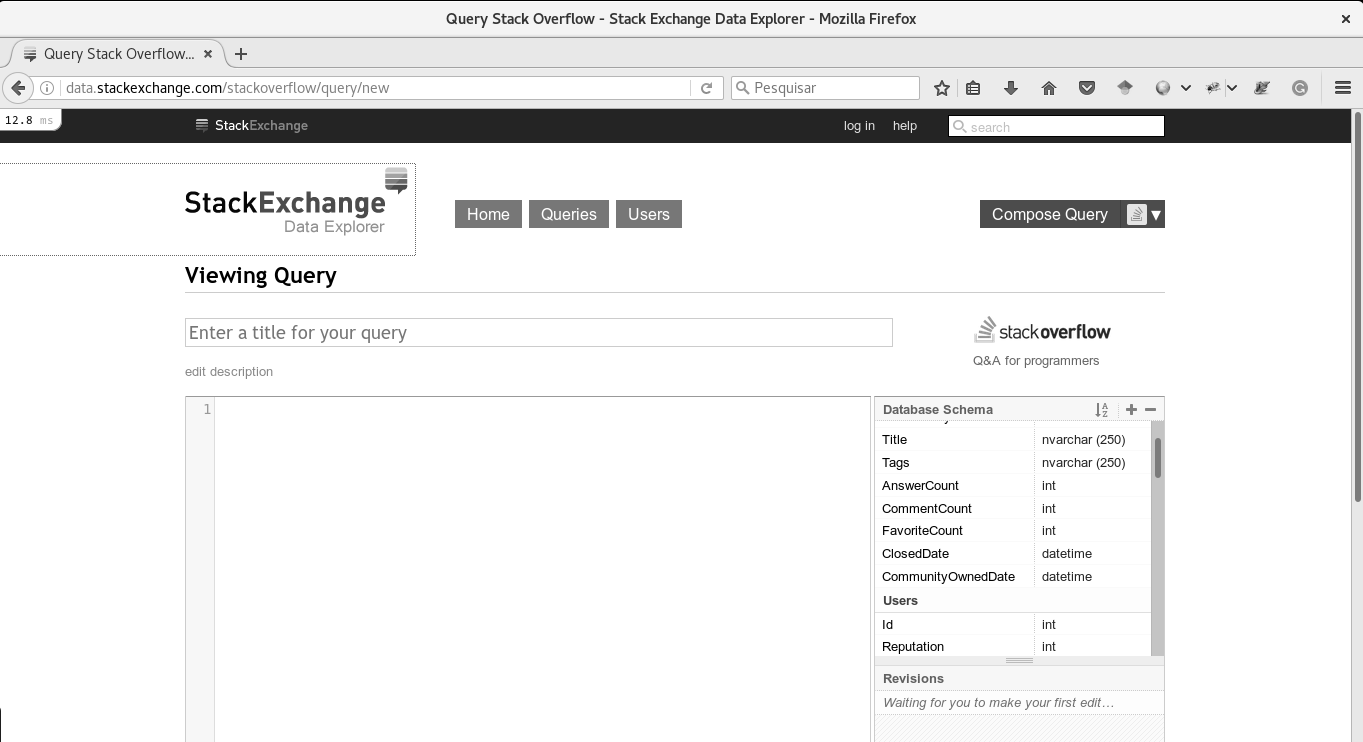
\includegraphics[width=0.8\linewidth]{./chapter-pesquisa-com-profissionais/img/stack-exchange.png}
	\caption{Ferramenta de coleta de dados da rede Stack Overflow}
\label{fig:stack-exchange}
\end{figure}

Para a fonte FA01 foi desenvolvido um Web Crawler para coletar as informações
dos participantes. Um Web Crawler (rastreador web) é um programa de computador
que navega pela World Wide Web de uma forma metódica e automatizada.  A partir
de uma lista de RMs previamente coletadas a ferramenta coletou os dados dos
participantes a partir do histórico de modificações da mesma. A
Figura~\ref{fig:historico-rm-python} apresenta o histórico de registros de uma
RM do projeto Python onde os dados dos participantes podem ser visualizados nos
quadros inseridos. A ferramenta utiliza uma marcação HTML e os seu valor de
classe (título, ou seja, nome de membro) para coletar os dados. Os dados
coletados também foram armazenadas em um banco de dados para posterior aplicação
de critérios de inclusão e exclusão.

\begin{figure}[htpb]
	\centering
	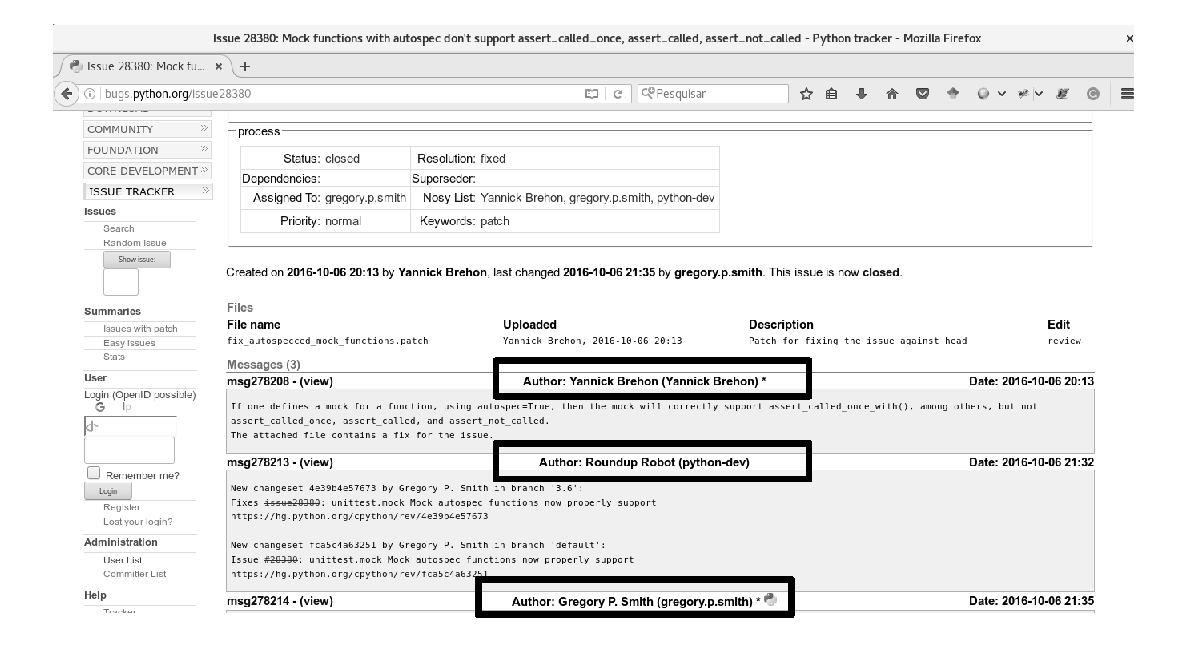
\includegraphics[width=0.6\linewidth]{./chapter-pesquisa-com-profissionais/img/historico-rm-python.pdf}
	\caption{Histórico de relatos de uma RM do projeto Python}
\label{fig:historico-rm-python}
\end{figure}

\subsubsection{Seleção dos Participantes}
\label{subsubsec:pesquisa_profissionais_plano_pesquisa}

Utilizamos estratégias distintas em cada fonte de amostragem para escolher os
potenciais participantes do levantamento. Para a fonte FA01 utilizamos os
registros históricos das RMs ocorridos nos últimos 05 anos. Além disso, foi
coletada a frequência que um participante teve algum tipo de interação com
projeto, como por exemplo abertura, solução ou comentários em RMs. Um
participante seria incluído caso tivesse pelo menos uma interação no período
avaliado.

No caso do Stack Overflow realizamos a busca de discussões que tinham relação
com as sentenças de busca descritas na Figura~\ref{fig:setencas-grupos}. Um
conjunto similar de sentenças de busca foi utilizado no mapeamento sistemático
descrito no Capítulo~\ref{ch:mapeamento-sistematico}. Para obtermos os dados
utilizamos a busca oferecida pelo próprio
site\footnote{\url{http://data.stackexchange.com/}}. Neste contexto, visando
restringir a seleção de grupos de participantes que estejam vinculados à
desenvolvimento e manutenção de software aplicamos as seguintes regras de
exclusão de participantes:

\begin{itemize}
	\item Proíbem expressamente a utilização dos seus dados, especialmente do
		seu endereço eletrônico, para a realização de estudos;
	\item A Fonte de Amostragem ao qual pertence não possui um mínimo de 05 anos
		de registros
	\item Para as discussões do Stack Overflow, aqueles que restringem
		explicitamente a mensagem individual entre seus membros;
    \item Utilizam uma língua diferente do inglês, tendo em vista que o idioma
		 é padrão em fóruns internacionais e apenas existiam uma versão em
		inglês e português para o questionário utilizados.
\end{itemize}

\begin{figure}[htpb]
	\centering
	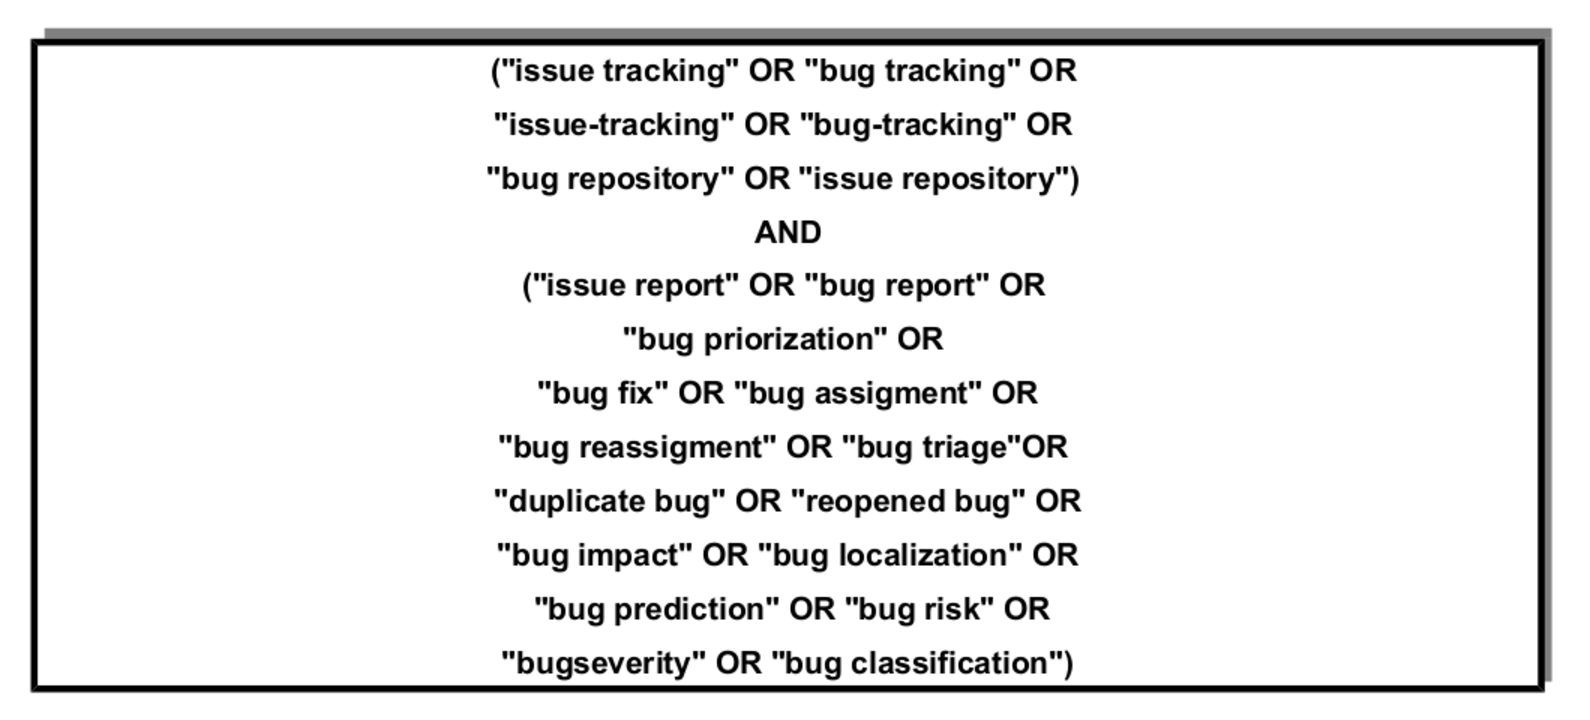
\includegraphics[width=0.8\linewidth]{./chapter-pesquisa-com-profissionais/img/setencas-grupos.pdf}
	\caption{Sentenças utilizadas para escolhas dos grupos do LinkedIn e de
		discussões no Stack Overflow}
\label{fig:setencas-grupos}
\end{figure}

\subsubsection{Questionário}
\label{subsubsec:questionario}

O formulário enviado aos participantes foi estruturado em três partes, cada uma
coletando um conjunto de informação. Na primeira parte estávamos interessados na
formação de base (background) do respondente. O segundo conjunto de perguntas
tinha por objetivo  coletar a percepção dos participantes sobre as
funcionalidades oferecidas pelas FGRMs\@. Na terceira parte estão as perguntas
sobre as melhorias e proposição de novas funcionalidades para as FGRMs que foram
propostas na literatura quando este trabalho foi realizado.

Antes de aplicarmos o formulário no público alvo foi realizado um processo de
avaliação constituído de quatro etapas. O formulário resultante de uma etapa foi
utilizado como entrada de outra imediatamente posterior. As etapas de avaliação
foram as seguintes:

\begin{enumerate}[(i)]
	\item Avaliação por Pesquisadores: Nesta etapa a primeira versão do
		formulário foi enviada para dois pesquisadores da área de manutenção de
		software.
	\item Avaliação por Profissionais: O formulário resultante da análise
		anterior foi encaminhado a dois profissionais que trabalham com
		manutenção de software.
	\item Piloto da Pesquisa: O formulário obtido da fase anterior foi utilizado
		em um piloto com dez profissionais envolvidos da manutenção de software
		de uma empresa pública de
		informática~-~PRODABEL\footnote{\url{{http://www.prodabel.pbh.gov.br}}}
	\item Tradução do Formulário: Em cada uma das etapas de anteriores o
		formulário foi aplicado em português, tendo em vista a falta de fluência
		em Inglês de alguns profissionais envolvidos no processo de avaliação,
		em especial na fase ``Piloto da Pesquisa'. Neste sentido, a última etapa
		consistiu na tradução do formulário para a língua inglesa. Esta etapa
		foi conduzida com  o suporte de um pesquisador experiente na área de
		Engenharia de Software.
\end{enumerate}

\subsubsection{Envio da Mensagem}
\label{subsubsub:envio_mensagem}

A fim de viabilizar e mitigar os riscos operacionais do envio manual de
mensagens ao participantes foi desenvolvido um processo automatizado de remessa
de mensagens aos participantes. O processo seguiu uma política que consiste em
enviar uma mensagem ao participante com base em um modelo. Após um um prazo de
dois dias uma nova mensagem era enviada. Foi construída uma lista para incluir o
endereço eletrônico daqueles que não gostariam de receber lembretes ou de
participar da pesquisa de modo a respeitar a privacidade do participante. As
mensagens foram preenchidas (uma a uma) e enviadas por meio de correio
eletrônico com base no seguinte modelo:

\fbox{\begin{minipage}{\textwidth}
Dear \{\{ nome do participante\}\}\!

I’m Vagner Clementino (\url{homepages.dcc.ufmg.br/~vagnercs}), Master Student at
Federal University of Minas Gerais, Brazil. I’m conducting a research,
supervised by Prof\. Rodolfo Resende \@-\@ \url{homepages.dcc.ufmg.br/~rodolfo}
concerned with improvements in Issue Tracking System. As part of them, we
planned and executed a survey aiming at to reaching a large-scale population of
researchers/practitioners interested on the improve the features of the Issue
Tracking Systems. Based on your area of interest, we kindly invite you to take
part in the following survey:

\{\{url do formulario\}\}

You were chosen because your relevant participation/contribution in \{\{nome da
fonte de amostragem\}\}\@-\@ \{\{url da fonte de amostragem\}\}. Your opinion is
essential to strength our findings. Please, help us accordingly to your
possibilities by answering this survey until \{\{data limite\}\}. As soon as we
conclude the data analysis, we will share the results with all participants and
the software engineering community. If you have already fulfilled this
questionnaire, please ignore this email.

Thanks in advance,\\
Vagner Clementino\\

\end{minipage}}

\section{Resultados}
\label{sec:analise_dados}

Neste seção apresentamos os resultados obtidos da aplicação do questionário.
Começamos com a análise do perfil dos respondentes. Em seguida, avaliamos o
nível de satisfação que os participantes possuem com as ferramentas que eles
utilizam. Posteriormente verificamos a adoção das metodologias propostas pelos
agilistas no processo de desenvolvimento e em especial da manutenção de
software.

\subsection{Perfil dos Participantes}
\label{sub:pesquisa_prof_perfil_dos_participantes}

Antes de apresentamos os resultado sobre as ferramentas, avaliamos o perfil dos
respondentes. Como pode ser observado na
Figura~\ref{fig:grafico_melhorias_fgrm_funcao_particantes} a função mais
frequente é a de desenvolvedor. Todavia, grande parte dos respondentes estão
diretamente vinculados ao desenvolvimento e manutenção de software, tanto que
mais de 80\% da amostrada é formada por desenvolvedores, engenheiros de
software, gerentes e arquitetos. Neste sentido, pelo menos no que tange à função
desempenhada, obtivemos um conjunto significativo de participantes.

\begin{figure}[htpb]
	\centering
	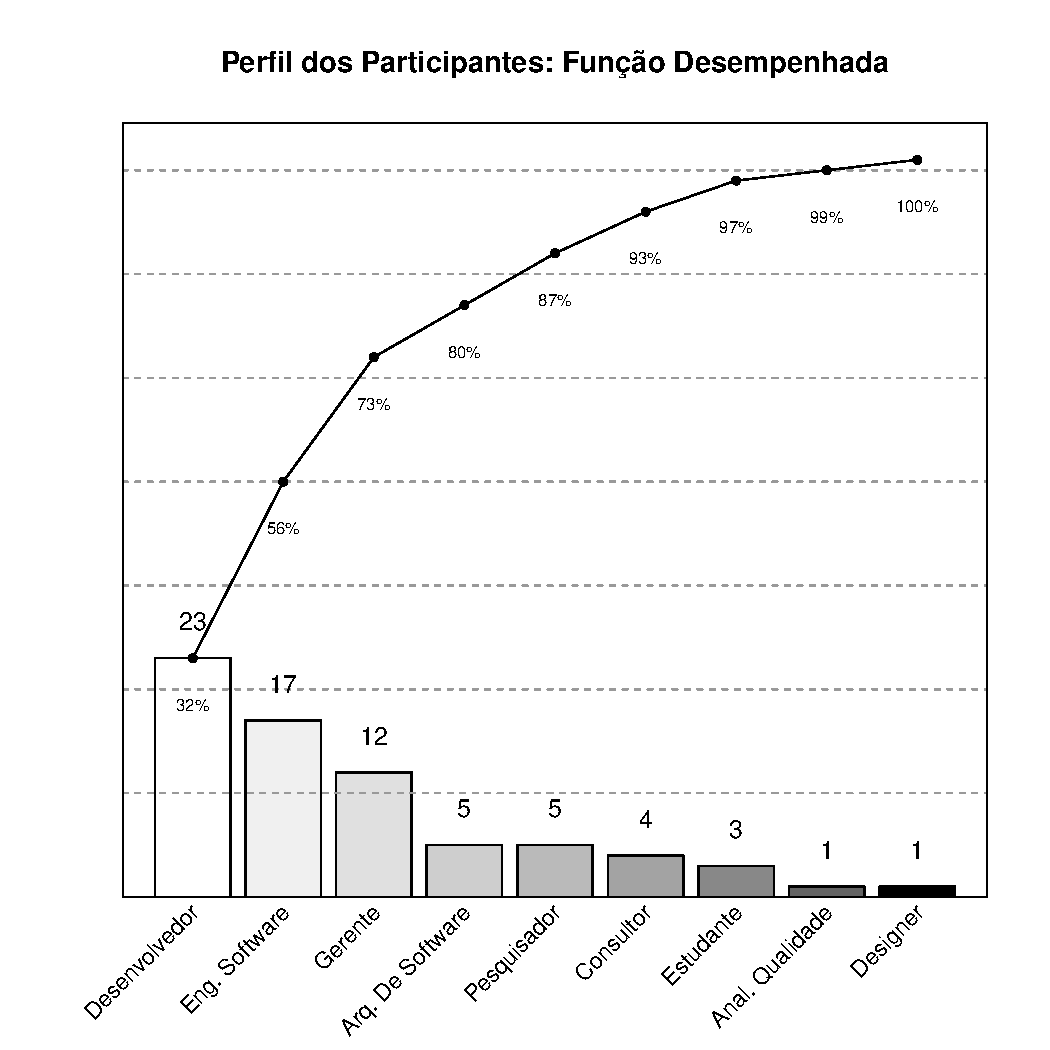
\includegraphics[width=0.6\linewidth]{./chapter-pesquisa-com-profissionais/img/grafico_melhoria_fgrm_funcao_participantes.pdf}
	\caption{Função dos Participantes}
\label{fig:grafico_melhorias_fgrm_funcao_particantes}
\end{figure}

A distribuição geográfica dos participantes pode ser visualizada na
Figura~\ref{fig:grafico_melhorias_fgrm_localizacao_geografica}. Há uma
proeminência de pessoas da Ásia e Europa e em seguida das Américas. Esta
distribuição pode minimizar possíveis enviesamentos que por ventura algum nicho
geográfico possa apresentar. Todavia, não está no escopo deste estudo discutir
as diferenças que a localização do participante pode influenciar aos resultados.

\begin{figure}[htpb]
	\centering
	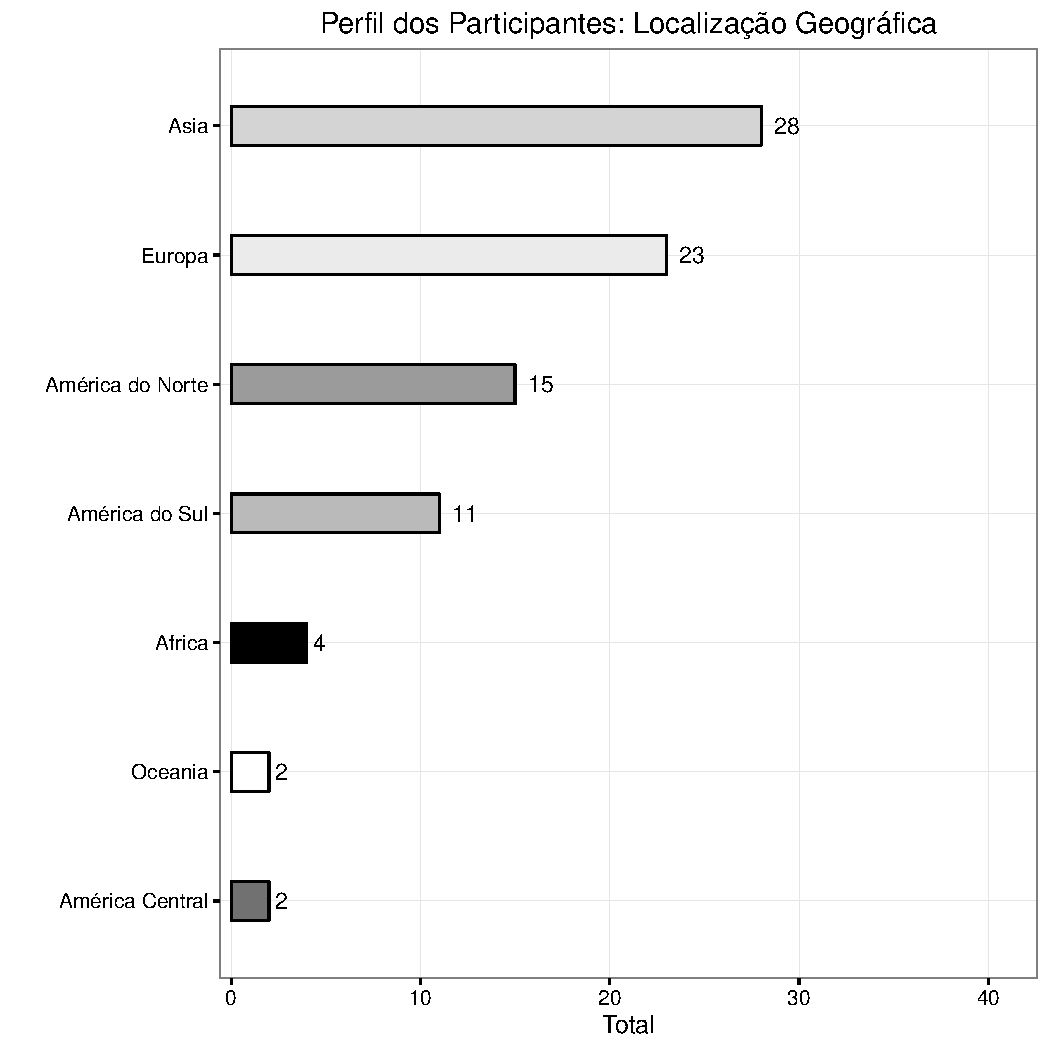
\includegraphics[width=0.8\linewidth]{./chapter-pesquisa-com-profissionais/img/grafico_melhorias_fgrm_localizacao_geografica.pdf}
	\caption{Localização Geográfica dos Participantes}
\label{fig:grafico_melhorias_fgrm_localizacao_geografica}
\end{figure}

Os respondentes trabalham em sua maioria em empresas privadas de software.
Existem também aqueles que participam de projetos de código aberto. A
distribuição do local de trabalho pode ser vista na
Figura~\cite{fig:grafico_melhorias_fgrm_local_trabalho}. É importante considerar
que grande parte dos respondentes pertencem à empresas privadas, onde os
processos e ferramentas não podem ser modificados pelo desenvolvedor. Esta
característica pode afetar os resultados, especialmente quando avaliarmos o
nível de satisfação das funcionalidades das FGRMs.

\begin{figure}[htpb]
	\centering
	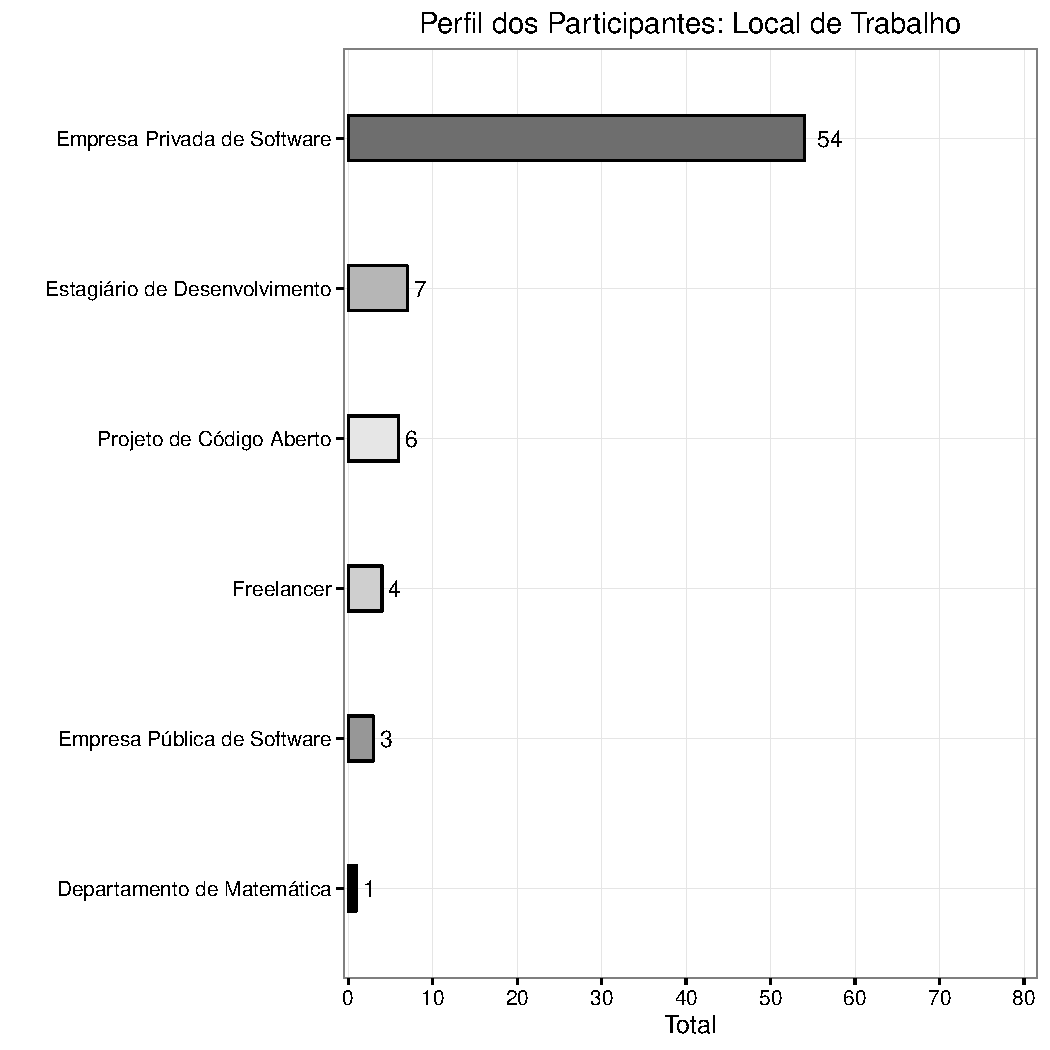
\includegraphics[width=0.8\linewidth]{./chapter-pesquisa-com-profissionais/img/grafico_melhorias_fgrm_local_trabalho.pdf}
	\caption{Local de Trabalho}
\label{fig:grafico_melhorias_fgrm_local_trabalho}
\end{figure}

No tocante ao tamanho da equipe verificamos a predominância de um número com
mais de seis membros, conforme pode ser observado na
Figura~\ref{fig:grafico_melhorias_fgrm_tamanho_equipe}. Apesar da maior
frequência de respostas é para equipes de tamanho maior do que dez membros,
acreditamos que o número de membros não seja muito maior do que isso.

\begin{figure}[htpb]
	\centering
	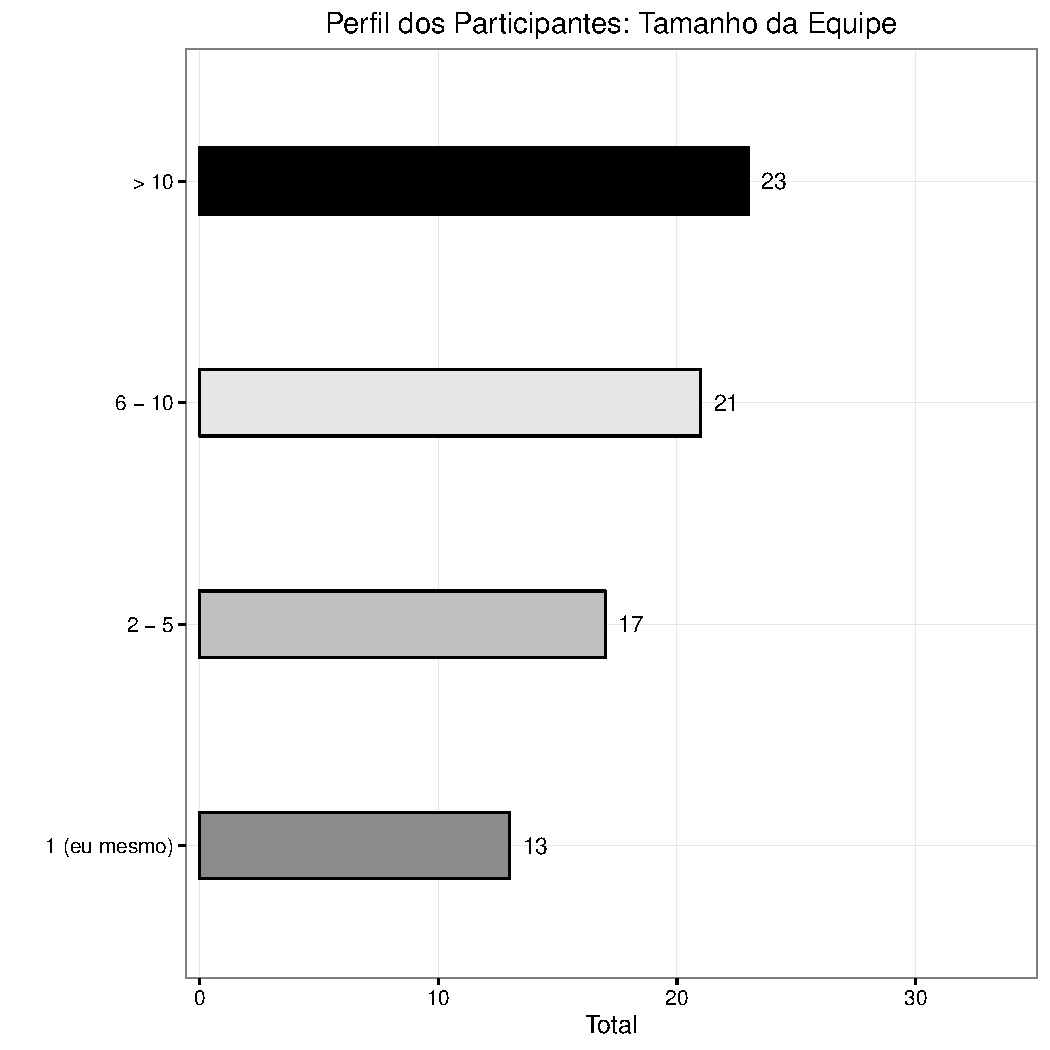
\includegraphics[width=0.8\linewidth]{./chapter-pesquisa-com-profissionais/img/grafico_melhorias_fgrm_tamanho_equipe.pdf}
	\caption{Tamanho da Equipe}
\label{fig:grafico_melhorias_fgrm_tamanho_equipe}
\end{figure}

Os participantes possuem com maior frequência entre três e dez anos de
experiência. Existem ainda um grupo significativo (09 participantes) que possuem
mais de dez anos trabalhando com desenvolvimento ou manutenção de software. Em
síntese, temos um grupo com significativa experiência o que pode agregar valor
aos resultados finais. A distribuição do tempo de experiência pode ser
visualizado na Figura~\ref{fig:grafico_melhorias_fgrm_tempo_experiencia}.

\begin{figure}[htpb]
	\centering
	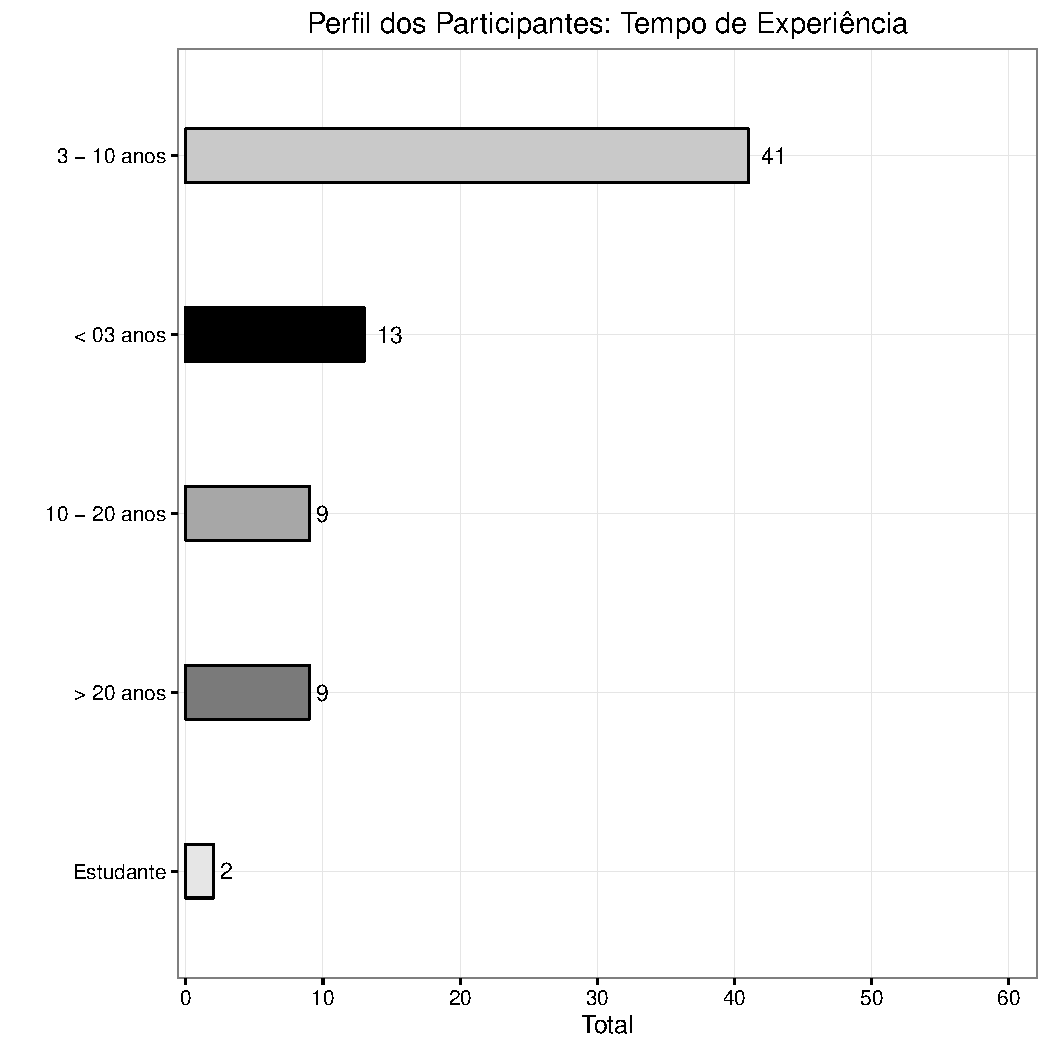
\includegraphics[width=0.8\linewidth]{./chapter-pesquisa-com-profissionais/img/grafico_melhorias_fgrm_tempo_experiencia.pdf}
	\caption{Tempo de Experiência}
\label{fig:grafico_melhorias_fgrm_tempo_experiencia}
\end{figure}

Em resumo as respostas vieram de desenvolvedores, localizados na Ásia e Europa,
com um tempo de experiência entre três e dez anos, trabalhando em uma equipe com
aproximadamente dez membros. A partir deste perfil entendemos que conseguimos
alcançar uma amostra com um perfil suficiente para responder as questões
propostas.

\subsection{Nível de Satisfação com as FGRM}
\label{sub:nivel_de_satisfação_com_as_fgrm}

Para respondermos as questões de pesquisa é importante analisarmos as
ferramentas utilizadas pelos profissional que respondeu a pesquisa. Esta
informação é importante tendo que vista que as opiniões dadas pelos
participantes estão diretamente relacionadas com a versão utilizada, podendo os
resultados se mostrarem diferentes se a pesquisa fosse realizada com outra
versão dos sistema.  A
Figura~\ref{fig:grafico_melhorias_fgrm_ferramentas_utilizadas} exibe as
ferramentas utilizadas pelos profissionais que responderam ao questionário. A
maior frequência ocorre para a ferramenta \textit{Jira} que é uma FGRM que
integra em seu processo de gestão das RMs métodos propostos pelos agilistas. Na
segunda posição visualizamos o Github que é um serviço de web para armazenamento
de projetos que usam o controle de versionamento \textit{Git} e possui uma FGRM
integrada.

\begin{figure}[htpb]
	\centering
	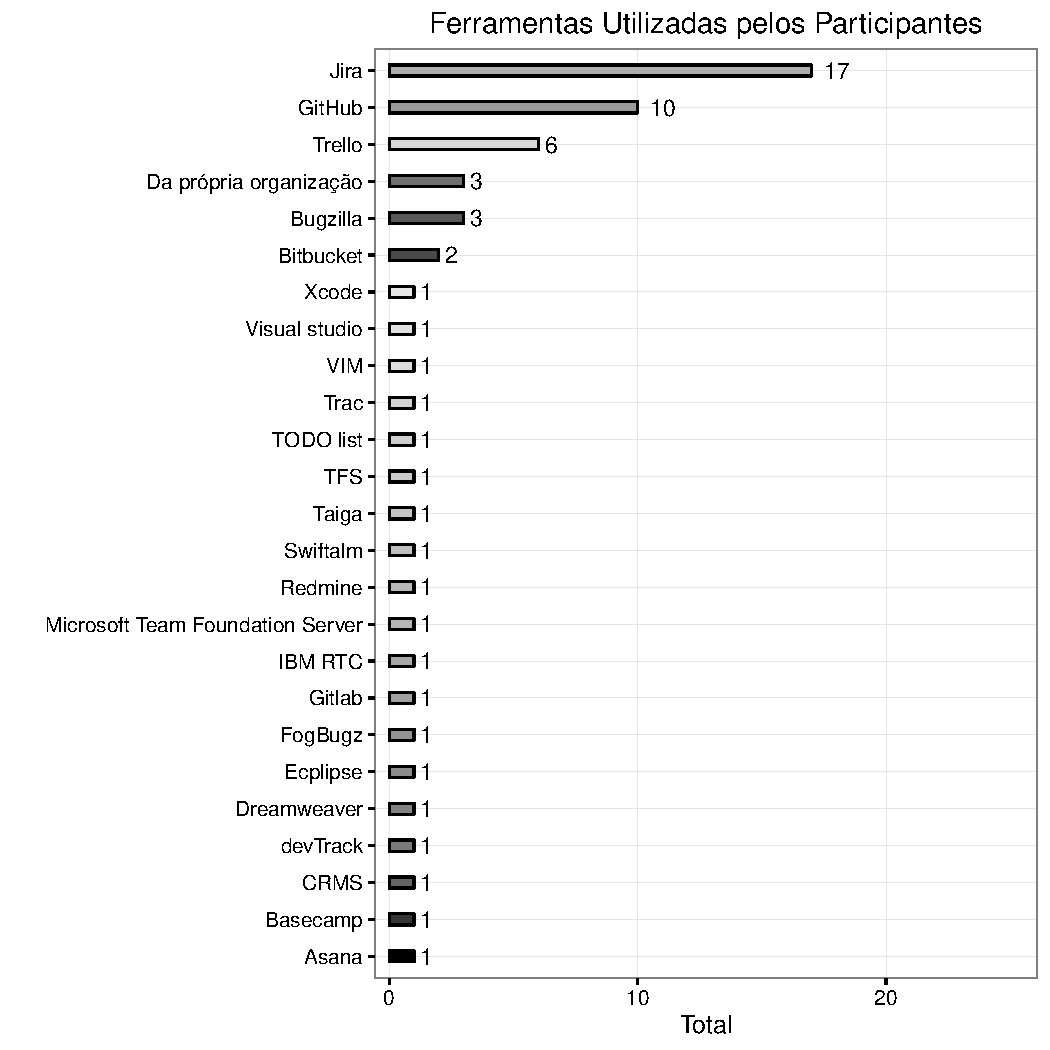
\includegraphics[width=0.8\linewidth]{./chapter-pesquisa-com-profissionais/img/grafico_melhorias_fgrm_ferramentas_utilizadas.pdf}
	\caption{Ferramentas utilizadas pelos participantes}
\label{fig:grafico_melhorias_fgrm_ferramentas_utilizadas}
\end{figure}

Inicialmente gostaríamos de saber qual o nível de satisfação dos participantes
com as funcionalidades oferecida(s) pela(s) FGRM(s) que ele utiliza atualmente.
Esta medida pode ser visualizada na
Figura~\ref{grafico_melhorias_fgrm_nivel_satisfacao}. Em grande parte os
respondentes estão satisfeitos com as funcionalidades. A resposta com maior
frequência foi \textit{OK}, o que pode representar que as FGRMs estavam, no
momento da realização deste estudo, atendendo as expectativas de seus usuários.
Este resultado não segue o que literatura da área discute, onde este tipo de
ferramenta é vista com necessidade de melhorias, tomando com base a visão dos
profissionais. Esta aparente dicotomia pode ser justificada, possivelmente, pelo
desconhecimento dos profissionais de funcionalidades que estão sendo propostas
na literatura que podem melhorar as suas atividades diárias.

\begin{figure}[htpb]
	\centering
	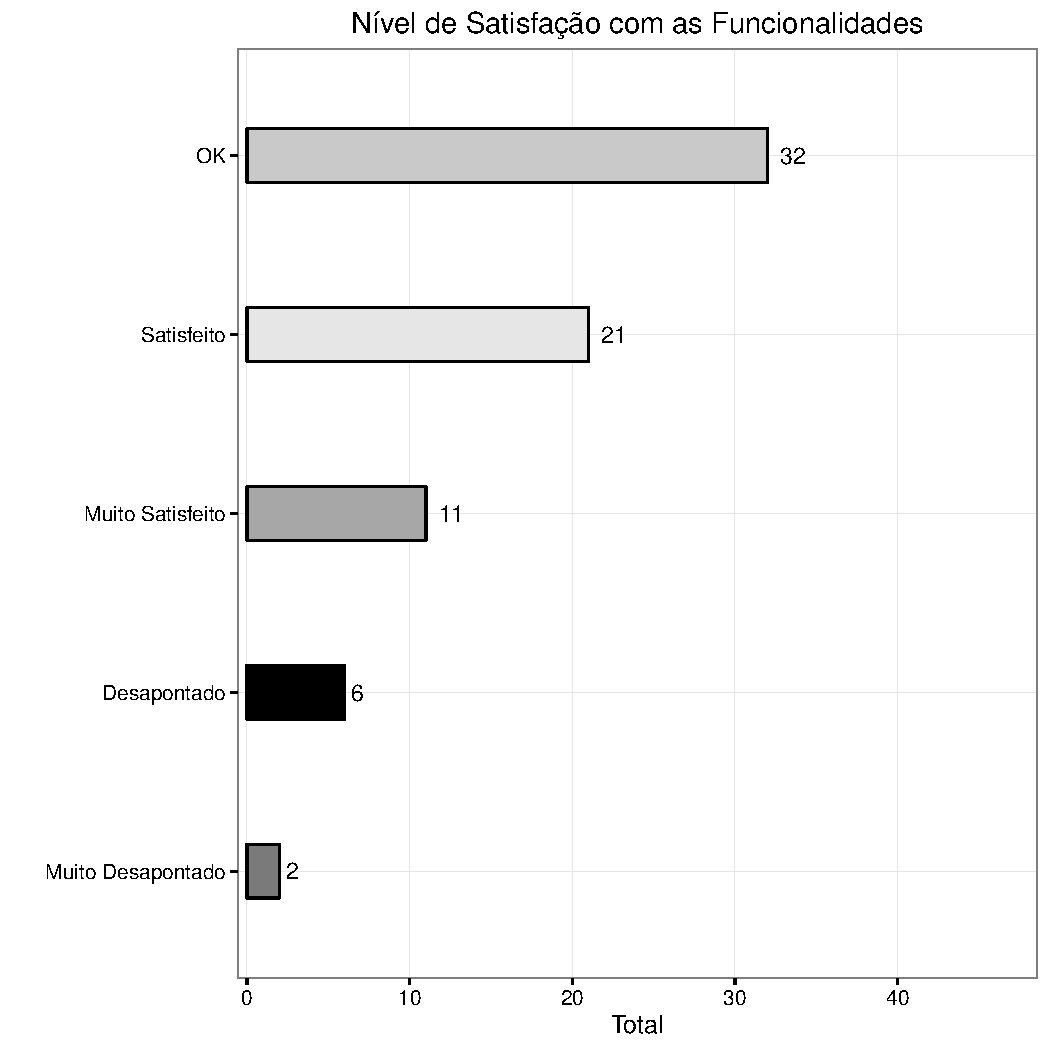
\includegraphics[width=0.8\linewidth]{./chapter-pesquisa-com-profissionais/img/grafico_melhorias_fgrm_nivel_satisfacao.pdf}
	\caption{Nível de satisfação com as Ferramentas}
\label{fig:grafico_melhorias_fgrm_nivel_satisfacao}
\end{figure}

No mesmo questionário verificamos se o respondente recomendaria a ferramenta que
utiliza para outro projeto. A probabilidade de recomendação é exibida na
Figura~\ref{fig:grafico_melhorias_fgrm_probabilidade_recomentacao}. De maneira
similar ao nível de satisfação grande parte dos participantes tendem a
recomendar a FGRM. Com base neste resultado, podemos deduzir que os
profissionais estão realmente satisfeitos com as funcionalidades da ferramenta
que utiliza ao ponto de recomendá-la.

\begin{figure}[htpb]
	\centering
	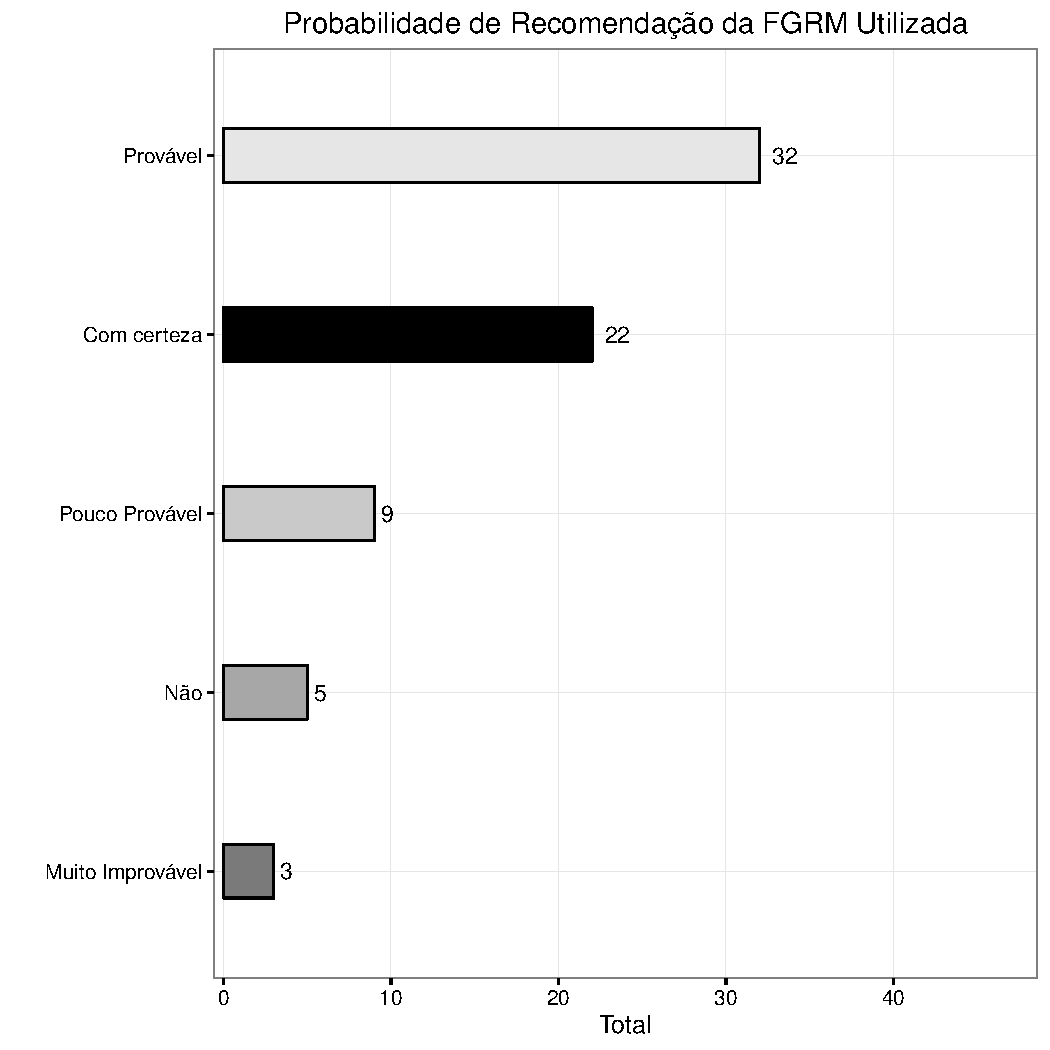
\includegraphics[width=0.8\linewidth]{./chapter-pesquisa-com-profissionais/img/grafico_melhorias_fgrm_probabilidade_recomentacao.pdf}
	\caption{Probabilidade de Recomendação da Ferramenta Utilizada}
\label{fig:grafico_melhorias_fgrm_probabilidade_recomentacao}
\end{figure}

\subsection{Avaliação das Funcionalidades Existentes}
\label{sub:avaliação_das_funcionalidades_existentes}

Nesta seção apresentamos a opinião dos profissionais sobre as funcionalidades
oferecidas atualmente pelas FGRM\@. O conjunto de funcionalidades apresentado ao
participante é o resultado do estudo descrito na
Seção~\ref{sec:caracterizacao_ferramentas}. Este ponto de vista pode ser
visualizado na Tabela~\ref{tab:avaliacao_funcionalidades}. É possível verificar
que os profissionais avaliaram como importantes funções tais como
\textit{Suporte ao Unicode, Múltiplos Projetos, Integração com Sistemas de
	Controle de Versão (VCS Integration)} como  funções importantes em sua
atividades diárias.

\begin{table}[htpb]
\centering
\resizebox{\textwidth}{!}{%
\begin{tabular}{@{}|l|ccccc|@{}}
\toprule
\multicolumn{1}{|c|}{\multirow{2}{*}{\textbf{Funcionalidade}}} & \multicolumn{5}{c|}{\textbf{Classificação}} \\ \cmidrule(l){2-6}
\multicolumn{1}{|c|}{} & \multicolumn{1}{c|}{\textbf{Not at all important}} & \multicolumn{1}{c|}{\textbf{Slightly Important}} & \multicolumn{1}{c|}{\textbf{Important}} & \multicolumn{1}{c|}{\textbf{Fairly Important}} & \textbf{Very Important} \\ \midrule
Documentation integration/generation, business reporting & 11 & 12 & 15 & 12 & 14 \\
Test planning integration & 11 & 13 & 13 & 13 & 9 \\
Customizable workflow & 9 & 14 & 21 & 14 & 15 \\
Unicode support & 9 & 9 & 21 & 16 & 24 \\
Custom fields & 5 & 17 & 25 & 22 & 8 \\
Support to Service Level Agreement & 14 & 22 & 15 & 13 & 10 \\
Plugin API to integration with other products & 8 & 14 & 21 & 19 & 16 \\
Multiple projects & 3 & 8 & 17 & 21 & 28 \\
Full-text search & 1 & 5 & 17 & 15 & 40 \\
File search & 4 & 15 & 18 & 17 & 24 \\
VCS integration & 7 & 16 & 16 & 13 & 21 \\
Multiples interfaces of notifications (E-mail, RSS, XMPP, etc) & 7 & 11 & 23 & 16 & 19 \\
Code Review Support & 2 & 2 & 0 & 0 & 5 \\
Ease of use & 0 & 2 & 2 & 0 & 1 \\
Integration with database \& app & 4 & 6 & 4 & 1 & 2 \\
Reviewing & 0 & 4 & 10 & 6 & 1 \\
User Experience and Ease of Use & 2 & 4 & 0 & 6 & 3 \\
Git branch style & 10 & 2 & 2 & 3 & 2 \\ \bottomrule
\end{tabular}%
}
\caption{My caption}
\label{tab:avaliacao_funcionalidades}
\end{table}

Por outro lado, apresentamos aos profissionais funcionalidades que poderiam ser
integradas à FGRM que ele utiliza. A opinião pode ser visualizada na
Figura~\ref{fig:ggrafico_melhorias_fgrm_melhorias}. Conforme pode ser observado
melhorias na busca de RMs, coleta de informações para solucionar na resolução da
RM e suporte ao registro de RMs foram avaliadas como funcionalidades que podem
melhorar as atividades do desenvolvedor.

\begin{figure}[htpb]
	\centering
	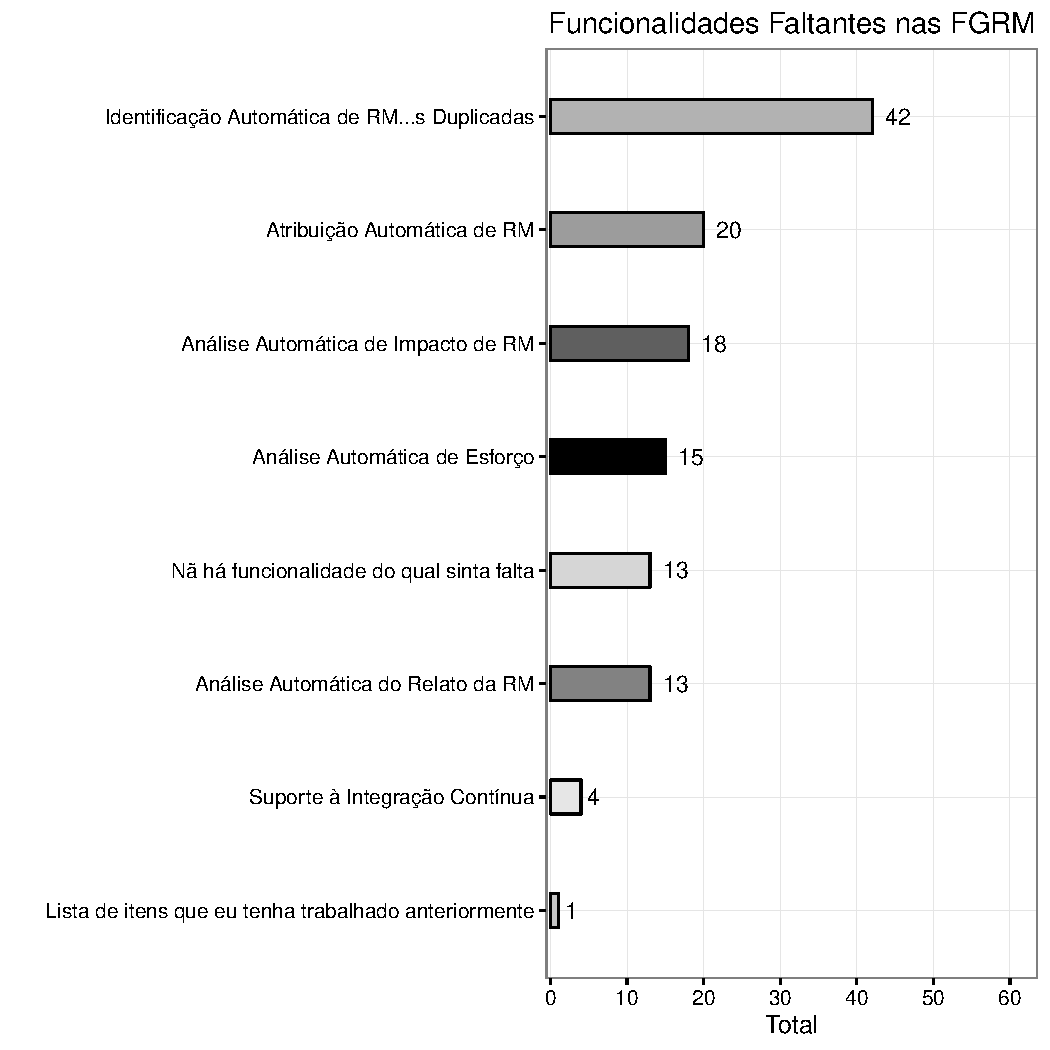
\includegraphics[width=0.8\linewidth]{./chapter-pesquisa-com-profissionais/img/grafico_melhorias_fgrm_funcionalidades_faltantes.pdf}
	\caption{Funcionalidades que o participantes sentem falta.}
\label{fig:grafico_melhorias_fgrm_funcionalidades_falantes}
\end{figure}

Algumas das melhorias propostas na literatura se mostraram interessantes pelos
profissionais. A
Figura~\ref{fig:grafico_melhorias_fgrm_funcionalidades_falantes} apresenta as
funcionalidades que os participantes sentem falta. Funções tais como
identificação automática de RMs duplicadas, atribuição automática de RM e
Análise de Impacto foram as mais frequentes.

\begin{figure}[htpb]
	\centering
	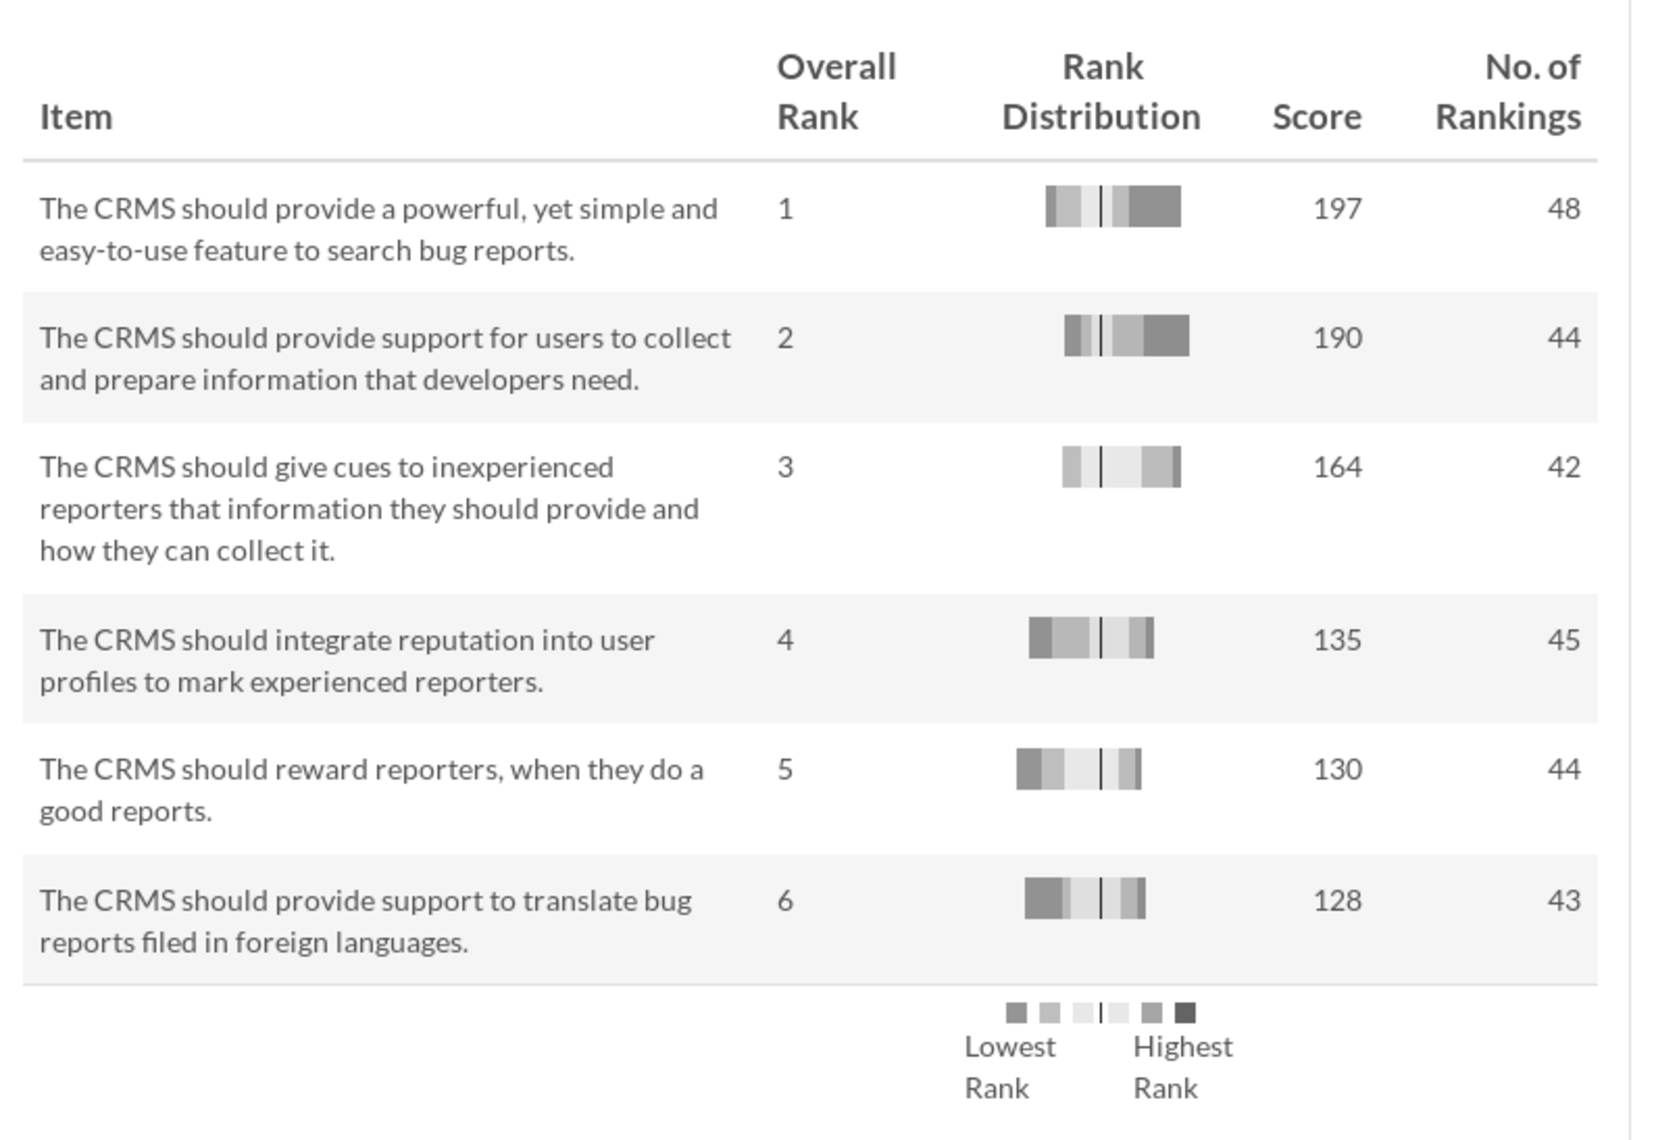
\includegraphics[width=0.8\linewidth]{./chapter-pesquisa-com-profissionais/img/grafico_melhorias_fgrm_melhorias.pdf}
	\caption{Novas funcionalidades para as FGRMs.}
\label{fig:ggrafico_melhorias_fgrm_melhorias}
\end{figure}

\subsection{Práticas Ágeis na Manutenção de Software}
\label{sub:práticas_ágeis_na_manutenção_de_software}

Nesta etapa do levantamento com profissionais, estamos interessados em analisar
como as práticas propostas pelos agilistas estão sendo utilizadas no
desenvolvimento e em especial na manutenção de software. A
Figura~\ref{fig:grafico_melhorias_fgrm_praticas_ageis_adotadas} exibe, segundo
os participantes, as práticas das metodologias ágeis que estavam sendo
utilizadas. Dentre elas, as mais adotadas foram Integração Contínua, Padrões de
Programação e Refatoração.

\begin{figure}[htpb]
	\centering
	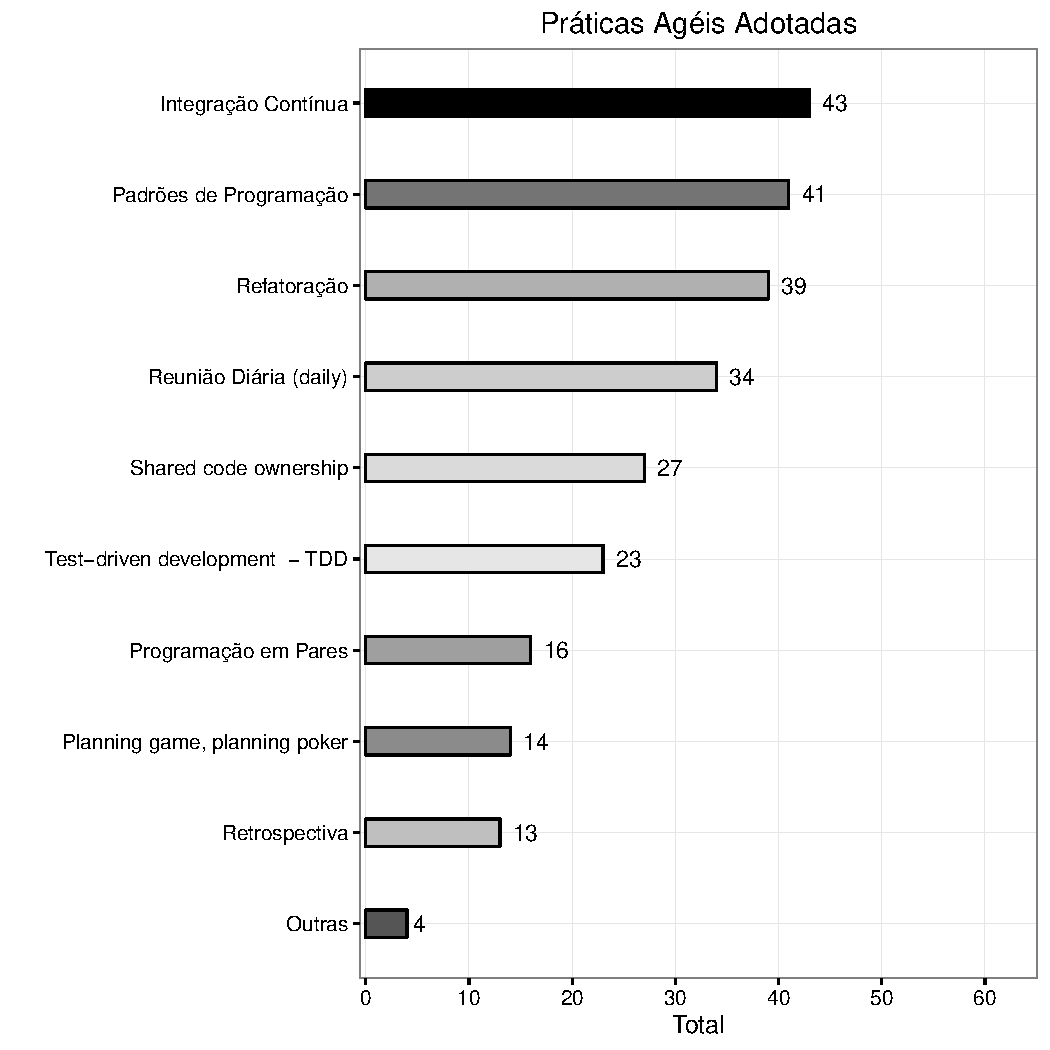
\includegraphics[width=0.8\linewidth]{./chapter-pesquisa-com-profissionais/img/grafico_melhorias_fgrm_praticas_ageis_adotadas.pdf}
	\caption{Metodologias propostas pelos agilistas que são adotadas pelos
		participantes.}
\label{fig:grafico_melhorias_fgrm_praticas_ageis_adotadas}
\end{figure}

A fim de avaliar como as FGRMs podem ajudar aos times de manutenção de software
na adoção das práticas propostas agilistas, apresentamos aos participantes do
levantamento uma lista de possíveis funcionalidades com este viés. A
Figura~\ref{fig:grafico_melhorias_fgrm_suporte_particas_ageis} apresenta a
opinião dos profissionais sobre as funcionalidades mais relevantes. Segundo
eles, a priorização automática de RMs urgente e não esperadas, ajuda do
desenvolvedor em sua reunião diária (daily) e o suporte a tarefas compartilhadas
foram as respostas mais frequentes.

\begin{figure}[htpb]
	\centering
	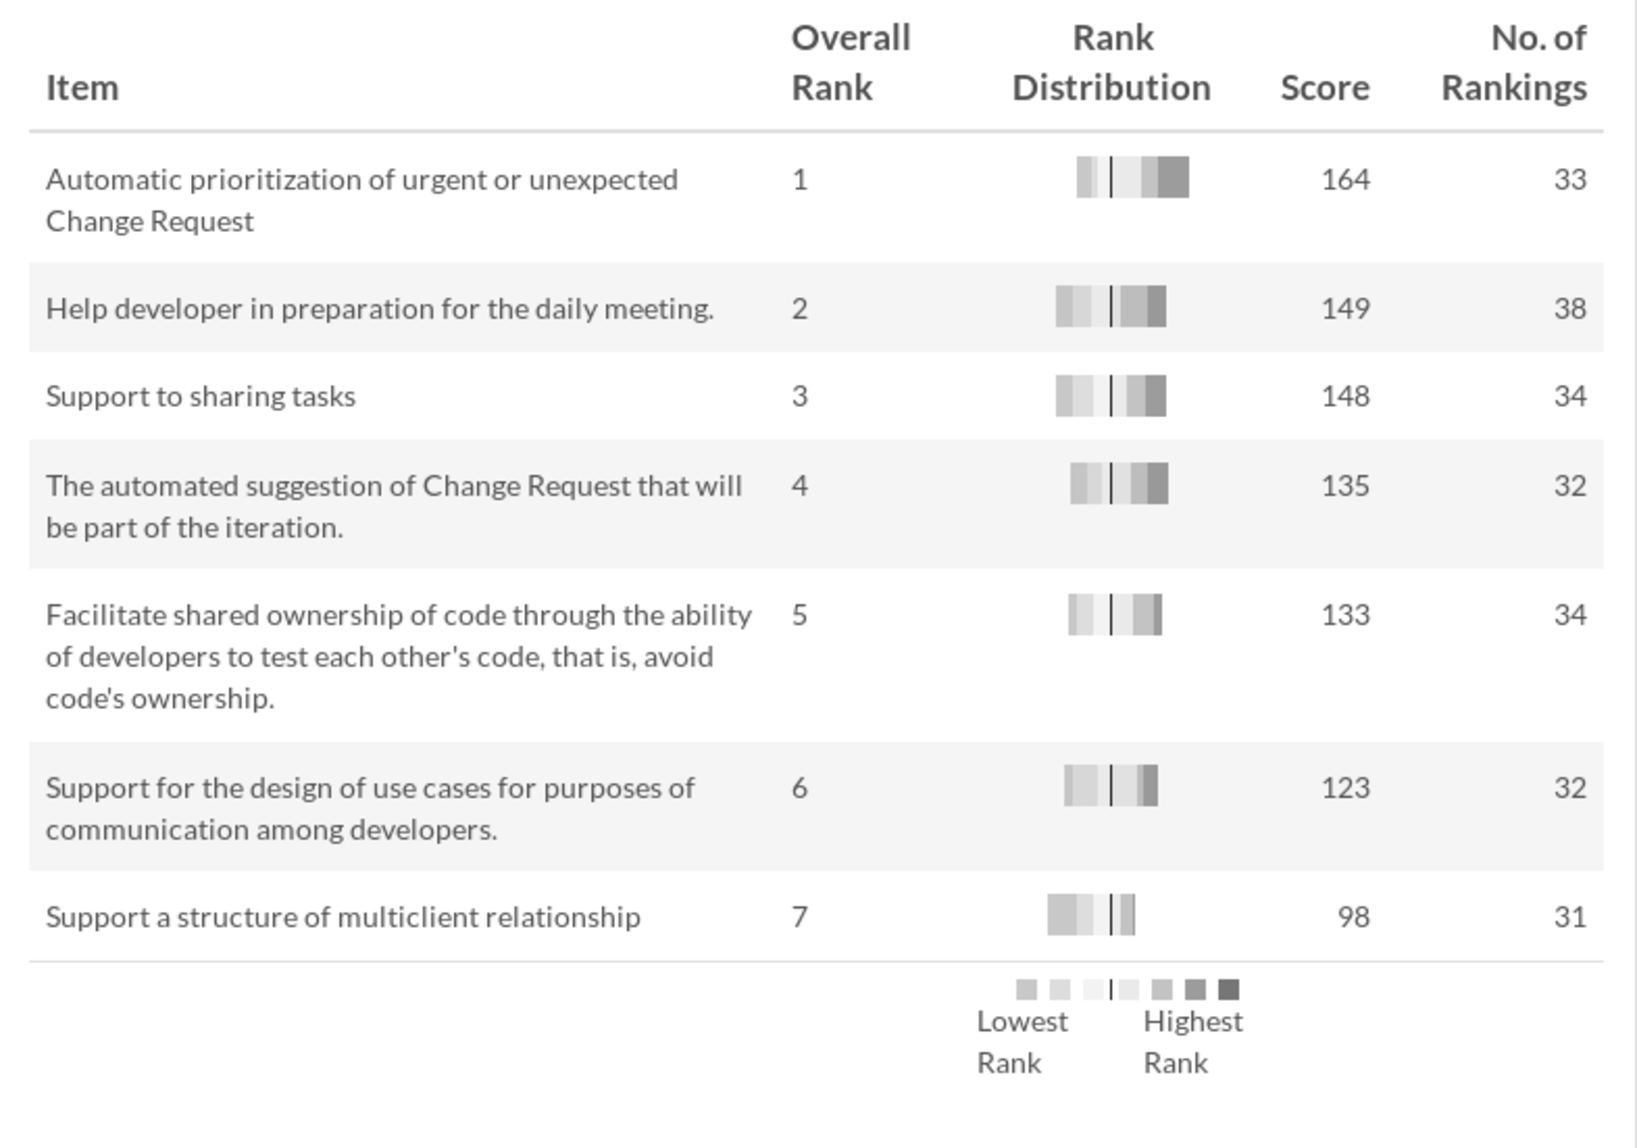
\includegraphics[width=0.8\linewidth]{./chapter-pesquisa-com-profissionais/img/grafico_melhorias_fgrm_suporte_particas_ageis.pdf}
	\caption{Classificação das funcionalidades que possam dar suporte ao uso das
	metodologias dos agilistas.}
\label{fig:grafico_melhorias_fgrm_suporte_particas_ageis}
\end{figure}

\section{Discussão}

\paragraph{Nível de Satisfação com a Ferramenta Utilizada:}
\label{par:pesq_profissionais_nivel_de_satisfação}

Em geral, o nível de satisfação com as funcionalidades oferecidas pelas FGRMs é
alto. Esta medida foi observada no
Figura~\ref{fig:grafico_melhorias_fgrm_nivel_satisfacao} no qual verificamos que
cerca de 90\% dos participantes estão de alguma forma satisfeito com a
ferramenta que utiliza. Este mesmo sentimento pode ser observado pela
relativamente alta probabilidade de recomendação da FGRM utilizada para um novo
projeto. Naquela medida verificamos que o mesmo percentual de participantes
pretendem recomendar o software que utiliza.

\paragraph{Funcionalidades Faltantes:}
\label{par:pesq_profissionais_funcionalidades_faltantes}

Apesar dos profissionais estarem satisfeitos com as fucionalidades ofertadas
pela FGRM que utiliza, quando lhe foi apresentado um conjunto de novas funções
grande parte dos participantes aprova a inclusão de algumas delas. Por exemplo,
certa de um terço dos participantes disseram sentir falta de um processo de
identificação automática de RMs duplicadas. Este resultado também foi encontrado
no trabalho de Bettenburg e outros~\cite{bettenburg2008makes} que ao conduzir um
levantamento com questionário onde o problema da duplicação de RMs foi descrito
com um dos problemas que pode atrapalhar o processo de solução da requisição.

Um outro ponto interessante a destacar é que as funcionalidades mais sentem
falta, também representam a maior quantidade de estudos na literatura. Posto de
outra forma, a automatização da detecção de duplicadas e atribuição de RMs são
os mais demandados e representam o maior número de trabalhos na literatura. Este
resultado pode sugerir a necessidade de divulgação do que está sendo proposto na
literatura tendo em vista que os profissionais se mostraram interessados nestes
tipos de funcionalidades.

\paragraph{Suporte às Práticas dos Agilistas:}
\label{par:pesq_profissionais_suporte_pratica_agilistas}

Apesar de ser pouco discutido na literatura, as FGRMs podem oferecer suporte às
praticas propostas pelos agilistas. Os participantes se mostrarem interessados
em funções tais como a priorização automática de RMs urgente e não esperadas,
ajuda do desenvolvedor em sua reunião diária (daily) e o suporte a tarefas
compartilhadas. Com a crescente adoção das práticas dos agilistas por times de
desenvolvimento e manutenção de software seria importante que este tipo de
ferramenta incorporasse em suas funcionalidades tal tendência. Segundo o nosso
atendimento e discutido na Seção~\ref{sec:caracterizacao_ferramentas} as FGRMs
estão longe de atender as demandas dos agilistas.

\section{Ameças à Validade}
\label{sec:pesquisa_profissionais_ameacas_validade}

A principal ameaça à validade deste trabalho está no numero de respondentes da
pesquisa. Apesar de ter sido realizada uma seleção metodológica de uma amostra
representativa da população o número de participantes limita a extrapolação do
resultados obtidos. O fato de ter sido utilizada uma amostragem de conveniência,
as generalizações são limitada já que amostra não verdadeiramente representa a
população. Por outra lado, utilizamos o arcabouço proposto por de
Mello~\cite{de2014towards} visando minimizar a introdução de viés na amostra
selecionada.

Ainda avaliando o processo de seleção das amostras utilizadas, não temos
garantia que as regras para seleção de participantes resultaram no conjunto mais
representativo da população. Vale ressaltar que todas as opiniões coletadas
devem sempre ser levadas em conta a ferramenta que o profissional utilizava
quando da aplicação do questionário.  Caso este mesmo estudo fosse realizado com
outras versões do mesmo sistema os resultados poderiam ser diferentes. Neste
sentido, a generalização dos resultados passa por esta característica do estudo.

\section{Resumo do Capítulo}
\label{sec:resumo_do_capitulo}
